\pdfminorversion=7
\documentclass[acmsmall,screen,review,anonymous]{acmart}

\usepackage{amsmath}
\usepackage{booktabs}
\usepackage{enumitem}
\usepackage{graphicx}
\usepackage{pifont}
\usepackage{tabularx}
\usepackage{xspace}
\usepackage{xcolor}

\setcopyright{none}
\settopmatter{printacmref=true,printccs=true,printfolios=true}
\renewcommand\footnotetextcopyrightpermission[1]{}

\newcommand{\sys}{SoftWall\xspace}
\newcommand{\QSU}{\textsc{QSU}\xspace}
\newcommand{\QSN}{\textsc{QSN}\xspace}
\newcommand{\MI}{\textsc{MI}\xspace}
\newcommand{\UQ}{\textsc{UQ}\xspace}
\newcommand{\NRx}{NeuralRx\xspace}
\newcommand{\kcj}[1]{\textcolor{red}{#1}}

\newtheorem{invariant}{Safety invariant}
\newtheorem{proposition}{Proposition}

\begin{document}

\title{SoftWall: Certifying Conditional Recovery for Shared-GPU AI-RAN}

\acmConference[SIGMETRICS '27]{ACM SIGMETRICS 2027}{June 7--11, 2027}{Atlanta, Georgia, USA}
\acmYear{2027}

\begin{CCSXML}
<ccs2012>
 <concept>
  <concept_id>10010520.10010521.10010537</concept_id>
  <concept_desc>Computer systems organization~Distributed architectures</concept_desc>
  <concept_significance>500</concept_significance>
 </concept>
 <concept>
  <concept_id>10010520.10010521.10010542</concept_id>
  <concept_desc>Computer systems organization~Real-time systems</concept_desc>
  <concept_significance>500</concept_significance>
 </concept>
 <concept>
  <concept_id>10003033.10003034.10003035</concept_id>
  <concept_desc>Networks~Network resources allocation</concept_desc>
  <concept_significance>300</concept_significance>
 </concept>
</ccs2012>
\end{CCSXML}

\ccsdesc[500]{Computer systems organization~Distributed architectures}
\ccsdesc[500]{Computer systems organization~Real-time systems}
\ccsdesc[300]{Networks~Network resources allocation}

\keywords{AI-RAN, GPU scheduling, neural receiver, conditional recovery, MPS, feasibility certificate}

\begin{abstract}
AI-and-RAN platforms seek to share a GPU between radio processing and external AI. NVIDIA
Multi-Process Service (MPS) enables concurrent execution, but it does not define a temporal contract
for the radio path. Optional neural reception introduces a further dependency: until the neural
outcome is known, the same transport block retains a conventional-recovery obligation that is absent
from the current GPU queue.

We present \sys, a runtime substrate that represents each unresolved obligation as recovery debt and
maintains an executable all-fail certificate. \sys refines this certificate through endpoint admission,
atomic outcome application, external-AI leasing, distributed ownership, and physical CUDA completion.
It also predicts a provenance-qualified feasibility envelope with four outcomes: safe and useful,
safe without AI slack, mandatory infeasible, and unqualified.

Two prespecified boundary states show that current idleness cannot provide this contract: debt-blind
admission can exceed the declared radio guard by 1-12~ms, while \sys rejected all 60 corresponding
requests before GPU launch. On two independent four-A100 nodes, a qualified warm path executed 4,800
actual TensorRT \NRx requests, 1,312 shared-cuPHY recoveries, 1,077 Qwen units, and 4,800 radio commits
without an observed deadline or invariant violation. The model matched an exact checker on 16,023
qualified states and predicted all 180 prespecified physical boundary rounds; a 64-debt certified
scheduler reached 1.494~ms p99 decision latency. A certificate-preserving recovery-first baseline
matched \sys at 385,262 timely tokens, and the full-bound sensitivity improved by only 0.066\%, below
the prespecified 5\% effect threshold. We therefore make no optimizer claim. These results qualify
finite-sample synthetic modes rather than production HARQ: the best 4.5~ms testMAC-target prototype
passed only 995/1,000 development requests, and External Aerial TDL-A remains unqualified. A separate
Sionna CDL-D/E holdout establishes conditional \NRx value only for its declared channel mode.
\end{abstract}

\maketitle

\section{Introduction}

AI-and-RAN consolidates radio physical-layer processing and external inference on shared accelerators.
The consolidation can reclaim idle GPU capacity, but it also couples a deadline-sensitive radio path
to kernels whose arrivals and execution times follow a different service objective. Existing systems
allocate GPU fractions, place requests across accelerator pools, reclaim reserved capacity, and split
background work into bounded units~\cite{yinyangran,cloudric,interplay,distributedairan}. The remaining
problem is not another allocation knob. It is a future mandatory job created by optional reception.

Consider one uplink transport block (TB). A timely \NRx result may improve its decoding outcome, while
failure, lateness, or lost evidence leaves conventional decoding mandatory. Before that outcome is
known, the conventional path is absent from the execution queue but remains part of the radio
contract. Several cells can hold this obligation at once, and several RAN homes can send recovery to
the same cuPHY lane. A scheduler that sees an idle GPU can therefore admit external AI into time that
must remain available for correlated recovery.

The obvious conservative response is to reserve every recovery until every neural outcome resolves.
That response preserves safety but discards capacity released by successful outcomes. The useful
middle ground requires a runtime to answer three questions together: which speculative paths may run,
which conventional jobs must remain executable under all-fail behavior, and which external-AI unit
can finish without invalidating that recovery plan. Queue occupancy, MPS percentage, and local
per-home admission do not represent all three.

\sys answers these questions with \emph{recovery debt}. Every unresolved optional path owns one debt,
and the runtime maintains a global executable all-fail certificate over those debts. A success deletes
one debt; failure, lateness, or missing evidence retains it. External AI receives a lease only when a
candidate recovery calendar and the complete AI transaction pass an independent verifier. This
construction makes MPS an execution mechanism, not the contract.

A mathematical certificate alone is insufficient. In our implementation, a valid calendar became
stale before kernel launch, simultaneous outcomes produced order-dependent intermediate states, a
fixed lease omitted launch control, and reply loss left ownership ambiguous. \sys carries the same
certificate through CUDA, IPC/P2P, and distributed-control state using bounded revalidation, atomic
outcome batches, physical latest-start enforcement, generation-safe ownership, and fence-confirmed
retirement. These mechanisms are established individually. Their combination refines an AI-RAN
recovery invariant from admission to physical completion.

The paper makes three connected contributions, followed by a physical validation:
\begin{enumerate}[leftmargin=*,itemsep=2pt]
  \item \textbf{Certificate-to-physical-execution refinement.} We derive seven requirements from
  measured counterexamples and bind a global recovery certificate to endpoint, transport, AI lease,
  worker epoch, completion fence, and single-commit state.
  \item \textbf{Predictive feasibility envelope.} We classify each qualified state as
  qualified-safe-useful (\QSU), qualified-safe-no-slack (\QSN), mandatory-infeasible (\MI), or
  unqualified (\UQ) before physical execution. A candidate scheduler never controls admission until
  an independent verifier accepts its certificate.
  \item \textbf{AI-RAN recovery-debt model.} We formalize same-TB optional reception, prove that one
  all-fail certificate covers every allowed failure subset, and show why current idleness cannot
  establish the radio contract.
  \item \textbf{Evaluation with negative results.} We exercise actual TensorRT \NRx, Aerial/cuPHY
  recovery, Qwen inference, CUDA IPC, NVLink P2P, MPS, and distributed faults. Strong safe baselines
  show no material AI-throughput headroom in the evaluated trace, which separates the substrate claim
  from an optimizer claim.
\end{enumerate}

\paragraph{Claim boundary.}
The guarantee is conditional on the qualified bounds and provenance of the evaluated mode. \sys does
not claim that MPS provides hard isolation, that finite-sample maxima are worst-case execution times
(WCETs), or that the synthetic timing contract is a production HARQ deadline. Five lifecycle subsets
are qualified or partially qualified and five remain \UQ; the claim does not require or imply a 10/10
lifecycle matrix.

\paragraph{Artifact plan.}
Upon acceptance, we will release the controller and verifier, finite-state and exact model checkers,
machine-readable protocols and analyzers, sanitized timing records, and manifests that bind source to
reported results through a long-lived archival repository. Proprietary Aerial/cuPHY, TensorRT, and
model components will be accompanied by acquisition and build instructions rather than redistributed.

\section{Background and Problem}

\subsection{AI-and-RAN on a shared GPU}

A shared accelerator exposes radio and external-AI kernels to the same execution and lifecycle state.
The hardware mechanism determines where kernels may run; a radio contract must additionally determine
which future work must remain executable.

\noindent\textbf{MPS Execution.}
MPS permits CUDA processes to execute concurrently and can limit a client's active-thread
percentage~\cite{nvidiampS}. It does not bound host scheduling, queueing, context lifecycle, allocation,
or arbitrary kernel blocking. Our diagnostics observe deadline misses under both tested caps and
separate the effect from a CPU-only sham in Section~\ref{sec:eval-mps}. We therefore use MPS to create
concurrency and place the admission contract above it.

\noindent\textbf{MIG-Off Reclamation.}
MIG provides spatial separation, but fixed partitions prevent one tenant from reclaiming another
partition's conditional capacity. We intentionally study MIG-off modes in which radio and external AI
can share qualified slack. A missing or failed bound classifies the mode as \UQ; the runtime never
imports a bound from another placement or lifecycle.

\subsection{Optional \NRx creates future mandatory work}

An optional receiver is speculative radio execution. It can improve the TB outcome, but it cannot
remove the requirement to produce a conventional result after failure, lateness, or lost evidence.

\noindent\textbf{Same-TB Dependency.}
Before the \NRx outcome resolves, conventional decoding is both conditional and mandatory under an
allowed future branch. It need not appear in a GPU queue. Static worst-case reservation protects this
branch but retains the reservation after timely neural success until the controller observes and
commits that outcome.

\noindent\textbf{Shared Recovery.}
Several cells can select \NRx together, and their failures can be correlated. Several RAN homes can
also send conventional work to one shared cuPHY lane. Per-home schedules do not compose on that lane;
the runtime must schedule the union of unresolved obligations.

\noindent\textbf{External-AI Admission.}
Qwen is a representative external workload that creates physical GPU contention. It is not an
AI-RAN-domain workload. Its request may run before unresolved recovery only when the complete
transaction, including launch control and physical completion, leaves an executable recovery plan.

Figure~\ref{fig:contract} shows the shared recovery path and one evaluated decision-boundary example.
It separates optional reception, conventional recovery, external AI, and the certificate that links
their physical completion.

\begin{figure}[t]
  \centering
  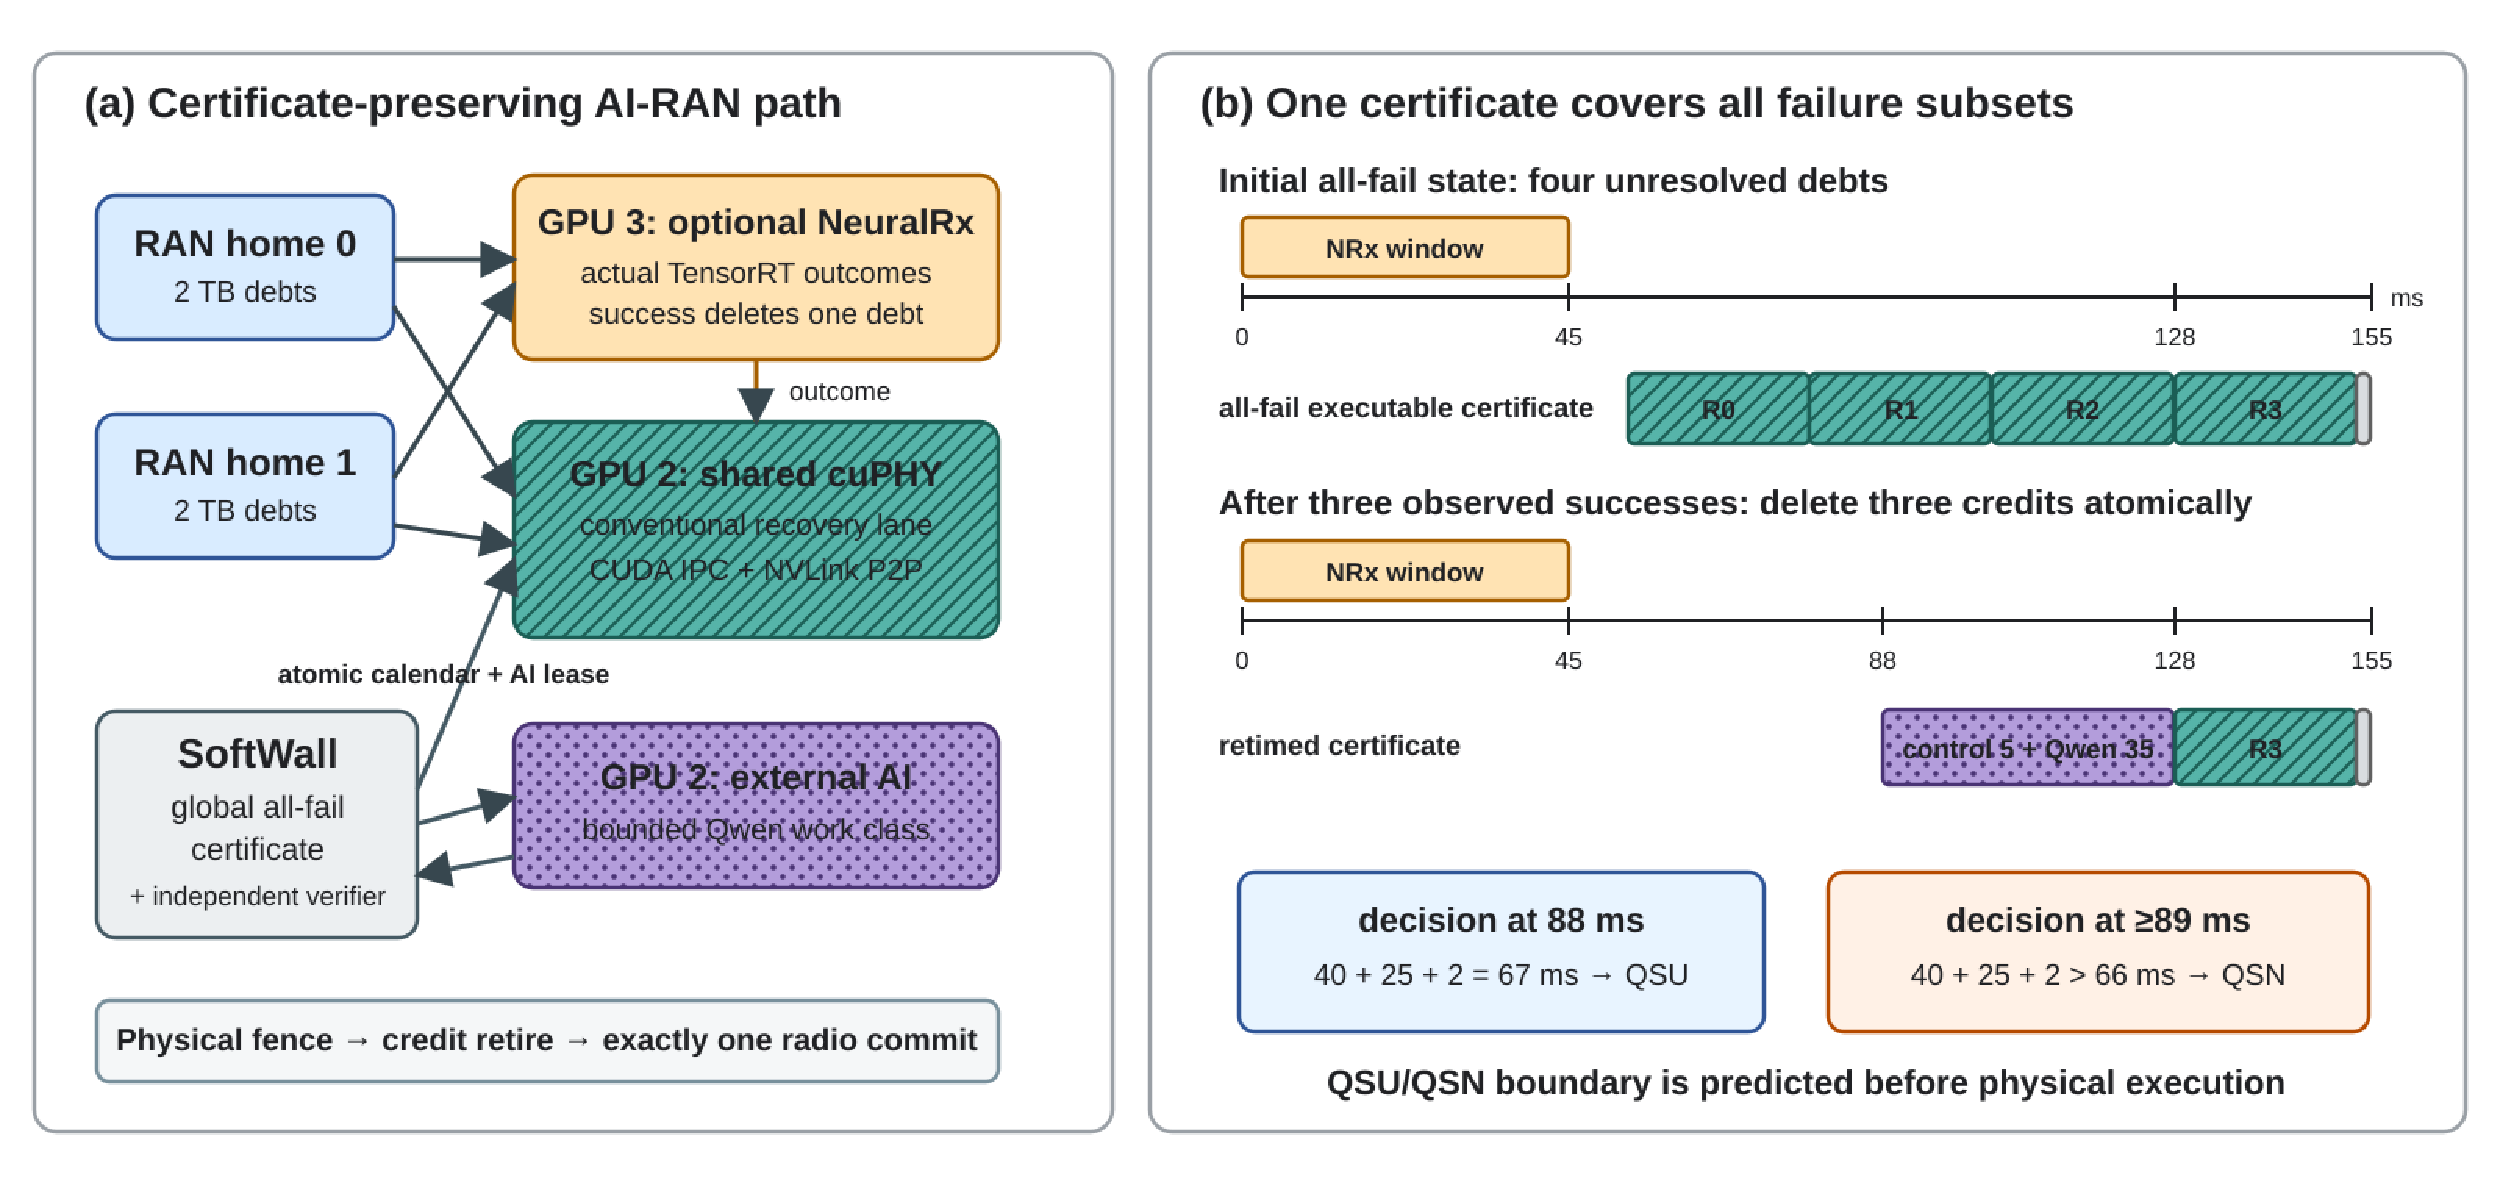
\includegraphics[width=\linewidth]{../../docs/current/figures/softwall_system_contract.pdf}
  \caption{Certificate-preserving AI-RAN path and one qualified boundary example. The all-fail
  schedule covers unresolved recovery, observed successes delete debt atomically, and external AI is
  admitted only when the remaining certificate stays executable.}
  \Description{Two RAN homes feed optional neural receiver paths and a shared conventional receiver.
  A timeline shows four initial recovery debts, three successes deleting debt, one retained recovery,
  and adjacent AI-admission decisions on opposite sides of the qualified boundary.}
  \label{fig:contract}
\end{figure}

\subsection{Threat model and qualification}

\sys provides a conditional guarantee for an explicitly qualified mode. Qualification binds service
bounds to the environment in which they were measured and defines the events the runtime must contain.

\noindent\textbf{Mode Provenance.}
A mode fixes GPU topology, MPS settings, process lifecycle, worker epoch, memory residency, co-run
class, software, and finite-sample whole-path bounds. Changing any element requires requalification.
The synthetic release period and result expiry used in evaluation are harness parameters, not NR slot
or production HARQ timing.

\noindent\textbf{Contained Events.}
The runtime handles \NRx failure and lateness, stale and duplicate messages, bounded reply loss before
or after a control-plane effect, missing AI replies after physical completion, and same-worker channel
reconnection. It fails closed when terminal physical evidence is absent.

\noindent\textbf{Excluded Events.}
Arbitrary GPU hangs, driver reset, unbounded host suspension, production-clock uncertainty, and
unqualified workloads remain outside the claim. Mandatory offered load without an all-fail schedule is
\MI rather than a reason to weaken the safety check.

\section{Failure-Derived Design Requirements}
\label{sec:requirements}

\sys uses known primitives: bounded admission, list scheduling, generation checks, CUDA fences,
IPC/P2P rings, and at-most-once ownership. The contribution is the refinement chain that connects
these primitives to one conditional-recovery invariant. Table~\ref{tab:counterexamples} names the
counterexamples and defers all measurements to Section~\ref{sec:evaluation}.

\begin{table}[t]
\caption{Counterexamples define the certificate-to-execution refinement chain.}
\label{tab:counterexamples}
\begin{tabularx}{\linewidth}{@{}p{0.25\linewidth}XX@{}}
\toprule
Counterexample & Broken assumption & Required refinement \\
\midrule
Local-safe/global-unsafe & Local certificates compose on a shared lane & Global obligation set and certificate \\
Dispatch tail & A certificate stays fresh until launch & Bounded revalidation and physical latest-start \\
Sequential cutoff replay & Simultaneous outcomes may apply in any order & Atomic outcome batch \\
Fixed AI lease & Execution time covers launch control & Control charge and AI blackout \\
Reply loss after effect & Retrying ambiguity is harmless & Generation quarantine and fail-closed admission \\
Two outstanding prepares & RPC at-most-once implies visible ownership & Single unlaunched-token invariant \\
Warm-bound reuse & Lifecycle does not affect service tails & Provenance-scoped qualification \\
\bottomrule
\end{tabularx}
\end{table}

\noindent\textbf{From Local to Global.}
Recovery feasibility belongs to the contended physical lane. The certificate must cover the union of
obligations before optional endpoint or external-AI admission.

\noindent\textbf{From Decision to Launch.}
A certificate must remain current through control delay, outcome observation, and CUDA launch. A
lease therefore includes launch control and carries an absolute latest-start enforced by the worker.

\noindent\textbf{From Logical Completion to Physical Retirement.}
RPC success is not CUDA completion, and reply loss is not proof that no effect occurred. Generations,
terminal markers, and physical fences bind ownership to retirement. The model in Section~\ref{sec:model}
defines this invariant, and the design maps it to executable components.

\section{Model}
\label{sec:model}

The model separates what the controller knows from what physical execution may still require. It
represents conditional work, qualified service, shared resources, and terminal evidence in one state.

\subsection{Jobs, modes, and provenance}

A job exposes only information available at admission. Runtime decisions cannot use future CRC,
future arrivals, realized service time, or a hidden channel label.

\noindent\textbf{Radio Jobs.}
A radio request is
\begin{equation}
  J_i=(r_i,d_i,h_i,c_i,K_i,q_i),
\end{equation}
where $r_i$ is release, $d_i$ result expiry, $h_i$ recovery home, $c_i$ the qualified conventional
host-to-commit bound, $K_i$ eligible \NRx endpoints, and $q_i$ optional radio value. Endpoint
eligibility includes its queue, transport, observation, and commit path under the active mode.

\noindent\textbf{External-AI Jobs.}
An external-AI request is
\begin{equation}
  A_a=(u_a,v_a,\ell_a,b_a,g_a),
\end{equation}
where $u_a$ is visible arrival, $v_a$ timely value, $\ell_a$ deadline, $b_a$ the qualified
physical-completion bound of its work class, and $g_a$ the guard before recovery. The controller may
select only from requests visible at the current event.

\noindent\textbf{Qualified Modes.}
Every bound carries provenance
\begin{equation}
 \pi=(\text{GPU},\text{placement},\text{MPS},\text{lifecycle},\text{co-run},\text{software}).
\end{equation}
A bound is admissible only when $\pi$ matches the active runtime. This rule prevents a warm or local
measurement from qualifying a cold, restarted, or remote path.

\subsection{Recovery debt and all-fail certificates}

An unresolved optional path creates work that may become mandatory. Recovery debt records that work
before any conventional kernel enters the queue.

\noindent\textbf{Debt.}
While outcome $i$ is unresolved, it induces
\begin{equation}
  R_i=(a_i(t),d_i-g_i,c_i,h_i),
\end{equation}
where $a_i(t)$ is the earliest legal recovery start at state time $t$. For unresolved set $U(t)$, an
all-fail certificate assigns every $R_i$ an interval $[s_i,s_i+c_i]$ that satisfies release, expiry,
resource capacity, and non-overlap. Any AI blackout or transport use that contends with recovery is
part of the same schedule.

\noindent\textbf{All-Fail Dominance.}
\begin{proposition}[All-fail dominance]
If a successful \NRx only deletes its conventional recovery and does not increase any remaining
job's demand, a feasible certificate for $U(t)$ is feasible for every failure subset
$F\subseteq U(t)$.
\end{proposition}
\begin{proof}
Delete the intervals of successful requests from the all-fail schedule. Releases, expiries,
capacities, and non-overlap of every retained interval remain unchanged.
\end{proof}

\noindent\textbf{Applicability.}
The reduction avoids enumerating $2^{|U|}$ outcome subsets. It does not apply if success creates new
mandatory work or changes another job's service bound. Such a mode requires a new certificate and
qualification.

\subsection{Global composition and atomic state}

The resource on which recoveries execute determines certificate scope. Logical ownership and physical
retirement must change with that certificate as one state transition.

\noindent\textbf{Composition.}
Certificates over disjoint recovery lanes compose by union. Certificates from homes that share one
lane do not compose independently. \sys therefore builds a global certificate over the union of their
obligations.

\noindent\textbf{State Transaction.}
The runtime state is
\begin{equation}
  X_t=(S_t,Q_t,T_t,L_t,E_t,C_t,G_t),
\end{equation}
where $S$ is the recovery schedule, $Q$ endpoint credits, $T$ transport generations, $L$ AI leases,
$E$ fences and worker epochs, $C$ radio commit state, and $G$ multi-home AI ownership. \sys constructs
a private candidate $X'$ and commits it only when
\begin{align}
\mathrm{VALID}(X') \equiv {}& \mathrm{ExecutableRecovery}(S') \land
 \mathrm{UniqueCredits}(Q',T') \nonumber\\
 &\land\ \mathrm{TimelyAI}(L',E') \land \mathrm{CurrentGenerations}(X').
\end{align}
A failed check leaves $X_t$ unchanged. A lease retires only through matching physical completion or a
qualified non-launch record.

\noindent\textbf{Safety Invariant.}
\begin{invariant}[Certificate-to-execution refinement]
For every admitted radio request, every allowed unresolved-outcome branch retains a collision-free
conventional path completing by expiry. No endpoint, transport, AI, or output credit is reused before
matching terminal physical evidence, and each request commits at most one radio result.
\end{invariant}

\subsection{Decision window and necessity}

The certificate defines the time window in which external AI may execute. The window depends on future
mandatory work, even when the physical lane is idle now.

\noindent\textbf{Safe AI-First Placement.}
Suppose $m_h$ equal-length recoveries are compacted at expiry $d_h$ with guard $g_h$. Let
$b_{\mathrm{eff}}$ include synchronous control, AI service, and completion guard. A sufficient
condition for AI-first execution is
\begin{equation}
 T_{\mathrm{dec},h}+b_{\mathrm{eff}}
 \le d_h-g_h-m_hc_h. \label{eq:window}
\end{equation}
The right side is the first recovery start retained by the certificate. This condition is
mode-specific and sufficient; it is not a general online optimum.

\noindent\textbf{Current Idleness.}
\begin{proposition}[Current idleness is insufficient]
Consider one non-preemptive recovery lane, common guard boundary $D$, unresolved recovery bounds
$c_1,\ldots,c_m$, and AI transaction bound $b_{\mathrm{eff}}$. If mandatory-only execution is
feasible but
\begin{equation}
  t+b_{\mathrm{eff}}+\sum_{i=1}^{m}c_i>D,
  \label{eq:debtblind}
\end{equation}
then a policy that admits AI from current idleness while ignoring unresolved recovery cannot guarantee
the radio contract.
\end{proposition}
\begin{proof}
Choose the allowed realization in which the AI transaction and every recovery take their declared
bounds. Non-preemptive execution places the last recovery after $D$ by
Equation~\ref{eq:debtblind}. Physical idleness at $t$ does not remove future mandatory demand.
\end{proof}

\noindent\textbf{Controller Choices.}
A conservative controller can preserve the initial certificate and drain recovery before AI. \sys
permits AI-first execution only with a new witness satisfying Equation~\ref{eq:window}. The evaluation
separates the necessity of this certificate from whether AI-first placement improves throughput.

\section{Design}
\label{sec:design}

The design maps each term in the safety invariant to a runtime component. No component can admit,
launch, retire, or commit work by consulting only its local queue.

\subsection{Overall architecture}

Figure~\ref{fig:contract} shows the architecture. The data path executes radio and external-AI work;
the control path maintains the certificate and transfers authority between physical workers.

\noindent\textbf{Radio Components.}
Each \textit{RAN Home} owns request release, expiry, and single-commit state. \textit{Optional NeuralRx}
executes speculative TensorRT reception on an eligible endpoint. \textit{Shared cuPHY} owns the
conventional-recovery lane used by all homes. The shared lane is why certificate scope follows the
physical resource rather than the home boundary.

\noindent\textbf{Certificate Components.}
\textit{SoftWall} stores recovery debt, calendars, endpoint and transport generations, leases, worker
epochs, and commit state. An \textit{Independent Verifier} accepts a candidate only after checking job
identity, release, service, expiry, lane capacity, non-overlap, AI blackout, and current generation.
The candidate scheduler cannot bypass this verifier.

\noindent\textbf{External-AI Component.}
\textit{External AI} receives a bounded work class, absolute latest-start, and lease generation. It
returns a physical fence or a qualified non-launch marker. This terminal evidence permits credit
retirement while keeping AI ownership and radio recovery in the same transaction.

\subsection{Radio admission and outcome transition}

The controller establishes a valid all-fail state before speculative execution and preserves it when
outcomes arrive. This ordering prevents optional work from consuming capacity needed by the mandatory
branch.

\noindent\textbf{Mandatory-First Admission.}
On radio release, \textit{SoftWall} reserves conventional recovery before considering
\textit{Optional NeuralRx}. An endpoint is eligible only when its whole-path bound fits the fallback
cutoff and it owns a generation-matching ring and transport credit. Rejection leaves the conventional
path intact.

\noindent\textbf{Atomic Outcome Batch.}
All outcomes observed at a common cutoff enter one transition. Timely successes delete their debts;
failure, lateness, and missing evidence retain debt. Sequential replay is forbidden because it can
construct an intermediate state that never existed and evaluate it at a later host time.

\noindent\textbf{Replanning.}
After applying the batch, \textit{SoftWall} rebuilds the unresolved calendar from the current time. It
may retime recovery intervals, but it cannot delete unresolved work or reuse a physical credit without
terminal evidence.

\subsection{AI lease and physical enforcement}

AI admission is a certificate update rather than a queue insertion. The update covers control delay,
physical execution, and the interval in which recovery must remain unobstructed.

\noindent\textbf{Atomic Replan and Lease.}
\textit{SoftWall} evaluates one candidate containing the retimed calendar and one AI lease. The
candidate commits only when recovery remains executable, the AI transaction meets its deadline and
recovery guard, credits are unique, and every generation is current. Failure restores the prior state
without a partial lease or calendar update.

\noindent\textbf{Launch-Time Revalidation.}
A certificate older than the qualified launch-control interval is discarded. \textit{External AI}
receives an absolute latest-start and emits a non-launch marker after that time. This rule closes the
interval between host admission and CUDA launch.

\noindent\textbf{Fence-Based Retirement.}
The executor performs only the next non-preemptive action named by the certificate. Matching CUDA
completion retires buffers, transport credits, and leases. A host timeout without physical evidence
quarantines ownership and blocks new optional admission.

\subsection{Distributed ownership and fault containment}

One global AI queue may serve several RAN homes. \sys keeps ambiguity local while allowing qualified
mandatory radio work and unaffected homes to continue.

\noindent\textbf{Single Unlaunched Token.}
Prepare creates at most one unlaunched token per home. Commit grants launch authority only after local
and global certificates are current. A second prepare cannot create another broker-held token for the
same ownership epoch.

\noindent\textbf{Ambiguous Effects.}
Reply loss after a broker-side effect does not trigger a fresh retry. The home quarantines the token,
closes new AI admission, and waits for a current terminal marker. Stale and duplicate replies cannot
retire a newer generation.

\noindent\textbf{Lifecycle Boundary.}
Prepare, abort, commit, and complete carry generations and bounded markers in the qualified
same-worker reconnect mode. Full worker replacement and durable reconciliation require another
mechanism and remain \UQ.

\subsection{Feasibility classification}

Classification makes the contract operational before physical execution. Safety, usefulness,
overload, and missing evidence are distinct outcomes.

\begin{table}[t]
\caption{Predictive feasibility classes.}
\label{tab:classes}
\begin{tabularx}{\linewidth}{@{}lX@{}}
\toprule
Class & Meaning \\
\midrule
\QSU & All-fail recovery is executable and at least one qualified AI unit is admissible. \\
\QSN & All-fail recovery is executable, but the candidate AI unit cannot safely fit. \\
\MI  & The mandatory all-fail schedule is infeasible under known bounds. \\
\UQ  & A required bound or lifecycle provenance is absent or failed qualification. \\
\bottomrule
\end{tabularx}
\end{table}

\noindent\textbf{Safe and Useful versus Safe without Slack.}
\QSU and \QSN share a valid radio certificate. They differ only in whether the visible AI candidate
fits. This distinction exposes conditional capacity without weakening radio admission.

\noindent\textbf{Infeasible versus Unqualified.}
\MI is a proved scheduling result under known bounds. \UQ reports insufficient authority to apply
those bounds. \sys fails closed for \UQ even when unqualified sample timing appears to fit.

\section{Implementation}
\label{sec:implementation}

The prototype binds the model to persistent CUDA workers and explicit control objects. Its purpose is
to make certificate state observable and enforceable across process and GPU boundaries.

\subsection{Runtime topology}

The implementation runs with MIG disabled and MPS enabled. RAN homes, neural endpoints,
conventional recovery, and external AI execute in separate persistent workers.

\noindent\textbf{Radio and AI Workers.}
Local and remote TensorRT \NRx workers hold preallocated bindings and CUDA graphs. Persistent
Aerial/cuPHY workers execute conventional recovery, while a Qwen2.5-1.5B worker executes bounded
prefill classes. Multi-home modes direct conventional work to one shared recovery GPU.

\noindent\textbf{Transport.}
CUDA IPC rings connect processes on one GPU, and NVLink P2P rings connect GPUs. Each slot carries a
request generation and physical completion state. Copy completion does not imply receiver or recovery
completion; the owning worker publishes a separate terminal fence.

\noindent\textbf{Controller.}
The controller stores recovery calendars, endpoint and transport credits, worker epochs, global AI
ownership, and single-commit state. Unix-domain RPC carries control messages, while CUDA-resident data
stays on IPC/P2P paths.

\subsection{Certificate engine}

The certificate engine separates schedule construction from admission authority. This separation
contains candidate-scheduler bugs and makes each decision independently checkable.

\noindent\textbf{Candidate Scheduler.}
The scheduler applies deterministic list orders to radio jobs and visible AI candidates. It emits a
complete schedule, ownership delta, and mode fingerprint. Exact search is used only as a small-state
oracle and is not an optimization contribution.

\noindent\textbf{Independent Verifier.}
The verifier checks job identity, release, qualified service, expiry, lane capacity, overlap, AI
blackout, credit uniqueness, and generation. The runtime cannot execute a candidate rejected by the
verifier. This interface also supports retrospective comparison against exact feasibility.

\noindent\textbf{Event Loop.}
The executor performs the first non-preemptive action in an accepted certificate, observes its
terminal event, and replans. It never reorders physical work from an unverified host-side queue.

\subsection{Measurement and mode separation}

Instrumentation distinguishes logical decisions, host progress, GPU execution, and physical
retirement. This distinction prevents a host timestamp from being reported as a kernel boundary.

\noindent\textbf{Recorded Events.}
The runtime records release, admission, dispatch, worker observation, CUDA completion, commit return,
request and payload identity, ring generation, worker epoch, and lease retirement. Nsight traces check
GPU ordering for selected modes.

\noindent\textbf{Python and Native Paths.}
The qualified C158-C162 path uses pyAerial with persistent workers. A later native C++ effort verifies
input-layout and decoder parity only. It is not timing-qualified and its measurements are never mixed
with the Python mode's service bounds.

\noindent\textbf{Artifact Binding.}
Source hashes, protocols, seeds, node exclusions, analyzer versions, failures, and result hashes are
preserved in manifests. Every empirical block in this paper maps to a machine-readable artifact and
field set.

\section{Evaluation Methodology}
\label{sec:methodology}

The evaluation tests the invariant before performance. It first asks whether the physical system
obeys the qualified contract, then whether the model predicts admission, and finally whether the
additional flexibility has measurable utility.

\subsection{Questions and metrics}

We organize the experiments around seven questions. Table~\ref{tab:rqs} connects each question to the
claim it can support.

\begin{table}[t]
\caption{Evaluation questions and their decision criteria.}
\label{tab:rqs}
\begin{tabularx}{\linewidth}{@{}lp{0.34\linewidth}X@{}}
\toprule
RQ & Question & Decision criterion \\
\midrule
1 & Is MPS itself the contract? & Misses under cap-only diagnostics reject the premise. \\
2 & Does the full path preserve the certificate? & Radio, recovery, AI, credit, and commit gates all pass. \\
3 & Does refinement contain specified faults? & State audit and physical fault classes preserve invariants. \\
4 & Does the envelope predict physical admission? & Exact, retrospective, and unopened-boundary decisions agree. \\
5 & Does certified construction scale? & No false-safe result; decision and verification remain bounded. \\
6 & Does AI-first retiming add timely value? & Prespecified effect threshold against a strong safe baseline. \\
7 & Where does qualification end? & Lifecycle, production timing, and channel gates retain failures. \\
\bottomrule
\end{tabularx}
\end{table}

\noindent\textbf{Safety Metrics.}
We count radio expiry misses, declared-bound violations, guard crossings, invalid certificates,
duplicate commits, stale generation acceptance, transport-credit reuse, and residual leases. Zero
observed events is reported as a finite-sample result rather than a probability or WCET claim.

\noindent\textbf{Utility Metrics.}
External-AI utility is deadline-compliant token value and completed request count. Radio utility is
correct TB outcome under the declared channel mode. Candidate-policy comparisons preserve the same
radio decisions and observable inputs.

\subsection{Testbed, workloads, and contract}

Authoritative campaigns use two independent nodes, each with four A100-SXM4-40GB GPUs connected by
NVLink. Facility identity is withheld for anonymous review. MIG is off and MPS is on.

\noindent\textbf{Radio and External AI.}
Radio execution uses NVIDIA Aerial/cuPHY and TensorRT \NRx. Qwen2.5-1.5B prefill creates external GPU
contention. BurstGPT supplies arrivals and token values from four non-overlapping public-trace
windows~\cite{burstgpt}; Qwen is not labeled an AI-RAN-domain workload.

\noindent\textbf{Qualified Synthetic Contract.}
The evaluated warm mode uses harness period/expiry \texttt{P180/D155}, with finite-sample whole-path
bounds $B_{\mathrm{NRx}}=45$~ms, $B_{\mathrm{conv}}=25$~ms,
$B_{\mathrm{AI}}(\text{context64})=35$~ms, and a 2~ms guard. The period is not an NR slot, and the
expiry is not a production HARQ deadline. Other AI contexts use their separately qualified work class.

\noindent\textbf{Channel Modes.}
Synthetic channels drive system qualification. A separate Sionna CDL-D/E mode tests radio value under
its own channel, radio, model, and precision contract. Aerial TDL-A and field IQ remain outside that
supported mode.

\subsection{Protocols and baselines}

Each authoritative campaign freezes its decision rule before opening the outcome. Development and
holdout runs use independent seeds and nodes where the gate requires them.

\noindent\textbf{Experimental Discipline.}
Protocols fix source hash, workload, bounds, seeds, node assignment, exclusions, analyzer, and stop
rule. Failed, negative, and \UQ runs stay in the ledger. A model-predicted boundary is frozen before
physical execution.

\noindent\textbf{Safe Baselines.}
\emph{Static global-safe} retains worst-case recovery reservation. \emph{Certificate-preserving
recovery-first} uses the same max-radio decisions, initial all-fail admission, arrivals, bounds,
workers, and single-commit rule as \sys, but drains unresolved recovery before external AI. \sys adds
AI-first placement only with a valid witness. The offline oracle sees the realized trace and supplies
an unattainable upper bound.

\noindent\textbf{Diagnostic Baselines.}
Debt-blind current-idle admission, local-only certificates, and uncontrolled MPS diagnose broken
assumptions. They are not safe performance comparators and are not used to claim throughput gains.

\paragraph{Reproducibility.}
The anonymous artifact package contains source, protocols, manifests, analyzers, exact checker,
independent verifier, result summaries, and figure builders. Hardware campaigns require proprietary
Aerial/cuPHY and TensorRT components; model, checker, trace, and analysis paths do not. Node names and
absolute paths are removed from the review artifact.

\paragraph{Use of generative AI.}
Generative-AI tools assisted with language editing, organization, bibliography normalization, and
consistency-checking scripts. The authors designed the system and model, fixed protocols, executed
experiments, inspected failures, and verified every claim against hashed artifacts. Generative AI
produced no experimental measurement or ground-truth label.

\section{Evaluation}
\label{sec:evaluation}

We report the experiments in claim order. Safety and prediction are primary outcomes; throughput and
production qualification are independent gates with negative results preserved.

\subsection{MPS is a mechanism, not the contract}
\label{sec:eval-mps}

RQ1 asks whether an active-thread cap can stand in for the radio contract. The answer is no for the
tested separate-client and lifecycle conditions.

% provenance: Q1_MPS_DIAGNOSTICS
\noindent\textbf{Cap-Only Diagnostic.}
A separate-client overrun produced 2/1,500 deadline misses at a 100\% cap and 1/1,500 at a 20\% cap.
Reducing active-thread percentage did not eliminate the tail.

\noindent\textbf{Lifecycle Control.}
A later matched comparison observed 0/10,000 misses for a CPU socket sham and 12/10,000 for the
GPU/MPS-client arm. The result isolates a GPU-client lifecycle effect from the control channel used to
trigger it.

\noindent\textbf{Answer to RQ1.}
These finite samples do not estimate a universal miss probability. They reject the premise that MPS
cap selection alone is the certificate. The remaining experiments retain MPS as the execution
mechanism and test \sys's contract above it.

\subsection{End-to-end variable-class qualification}

RQ2 asks whether the certificate survives actual \NRx, shared conventional recovery, external AI,
and radio commit. We evaluate independent development and holdout nodes under one frozen warm mode.

% provenance: Q2_WARM_PATH
\noindent\textbf{Qualified Workload.}
The \texttt{P180/D155} campaign ran 600 epochs on each node and admitted Qwen contexts from 16 to 512
tokens with class bounds $\{35,35,35,40,65,75\}$~ms. Table~\ref{tab:q2} reports physical work rather
than simulated service.

\begin{table}[t]
\caption{End-to-end variable-class qualification.}
\label{tab:q2}
\begin{tabular}{@{}lrrr@{}}
\toprule
Metric & Development & Holdout & Combined \\
\midrule
Epochs & 600 & 600 & 1,200 \\
Actual \NRx requests & 2,400 & 2,400 & 4,800 \\
Timely \NRx successes & 1,750 & 1,738 & 3,488 \\
Physical shared recoveries & 650 & 662 & 1,312 \\
Qwen completions & 544 & 533 & 1,077 \\
Radio commits & 2,400 & 2,400 & 4,800 \\
Deadline misses & 0 & 0 & 0 \\
\bottomrule
\end{tabular}
\end{table}

\noindent\textbf{Whole-Path Results.}
Maximum observed \NRx, recovery, and radio-commit paths were 18.123, 13.465, and 118.022~ms. Every
executed Qwen unit remained within its work-class bound. The certificate rejected 55 context-256 and
68 context-512 requests before launch when recovery debt left insufficient room. No Qwen kernel began
after its latest-start.

\noindent\textbf{Physical Execution and Answer to RQ2.}
Separate Nsight Systems campaigns on the same A100, MIG-off, MPS substrate verify physical rather than
host-only overlap. A profile of \NRx and Qwen contains 191 unique kernel-overlap segments totaling
8.932~ms across seven early-AI windows. A profile of early conventional and other-cell \NRx observes overlap in
12/12 windows totaling 12.309~ms. These small profiler-instrumented samples establish kernel
co-execution; they do not qualify co-run service bounds or the later end-to-end mode. In that frozen
end-to-end campaign, the two nodes executed 4,800 actual TensorRT neural-receiver requests, 1,312 shared-cuPHY recoveries,
1,077 Qwen units, and one commit for every radio request without an observed deadline, bound, guard,
credit, or commit violation. This is a finite-sample qualification of the declared warm mode.

\subsection{Fault closure}

RQ3 asks whether logical recovery remains bound to physical ownership when messages are stale,
duplicated, delayed, or lost. We combine finite-state checking with physical fault injection.

% provenance: C160_FAULT
\noindent\textbf{State Audit.}
A finite-state audit checked 51 combinations of epoch, generation, fence, and marker state with no
invariant violation. It covers transitions that are difficult to time physically, including reply
ambiguity before and after an effect.

\noindent\textbf{Physical Fault Campaign.}
The A0-A6 campaign covers clean operation, correlated \NRx failure, reply delay before and after
physical completion, stale and duplicate responses, terminal channel fault, and post-fault
continuation. Across qualified nodes it executed 700 epochs, 2,800 actual \NRx requests, 942 shared
recoveries, and 2,800 radio commits with no observed deadline miss. It included 40 stale/duplicate
replay pairs, four terminal channel faults, and 260 continuation epochs after terminal fault.

\noindent\textbf{Fail-Closed Scope.}
One additional node violated the \NRx whole-path bound. We retained it as \UQ and did not pool it into
the passing result. The evidence supports containment only for the qualified fault and lifecycle
classes.

\subsection{Predicting an unopened physical boundary}

RQ4 tests whether the envelope predicts admission before observing a new physical outcome. We compare
analytic, exact, retrospective, and prespecified physical decisions.

% provenance: C162_ENVELOPE
\noindent\textbf{Model Agreement.}
The envelope matched exact feasibility on 16,023 qualified states and matched all 1,200 retrospective
physical decisions. We then froze seven boundary cases, their order, and node-specific seeds before
execution.

\noindent\textbf{Physical Boundary.}
Across two independent nodes and 180 rounds, model and runtime agreed in all 180. The campaign executed
720 actual \NRx requests, 330 recoveries, 90 Qwen units, and 720 commits with no observed deadline
miss. Context-64 at the conservative integer decision time of 88~ms was admitted in 30/30 rounds;
89~ms or later was rejected in 30/30.

\begin{figure}[t]
  \centering
  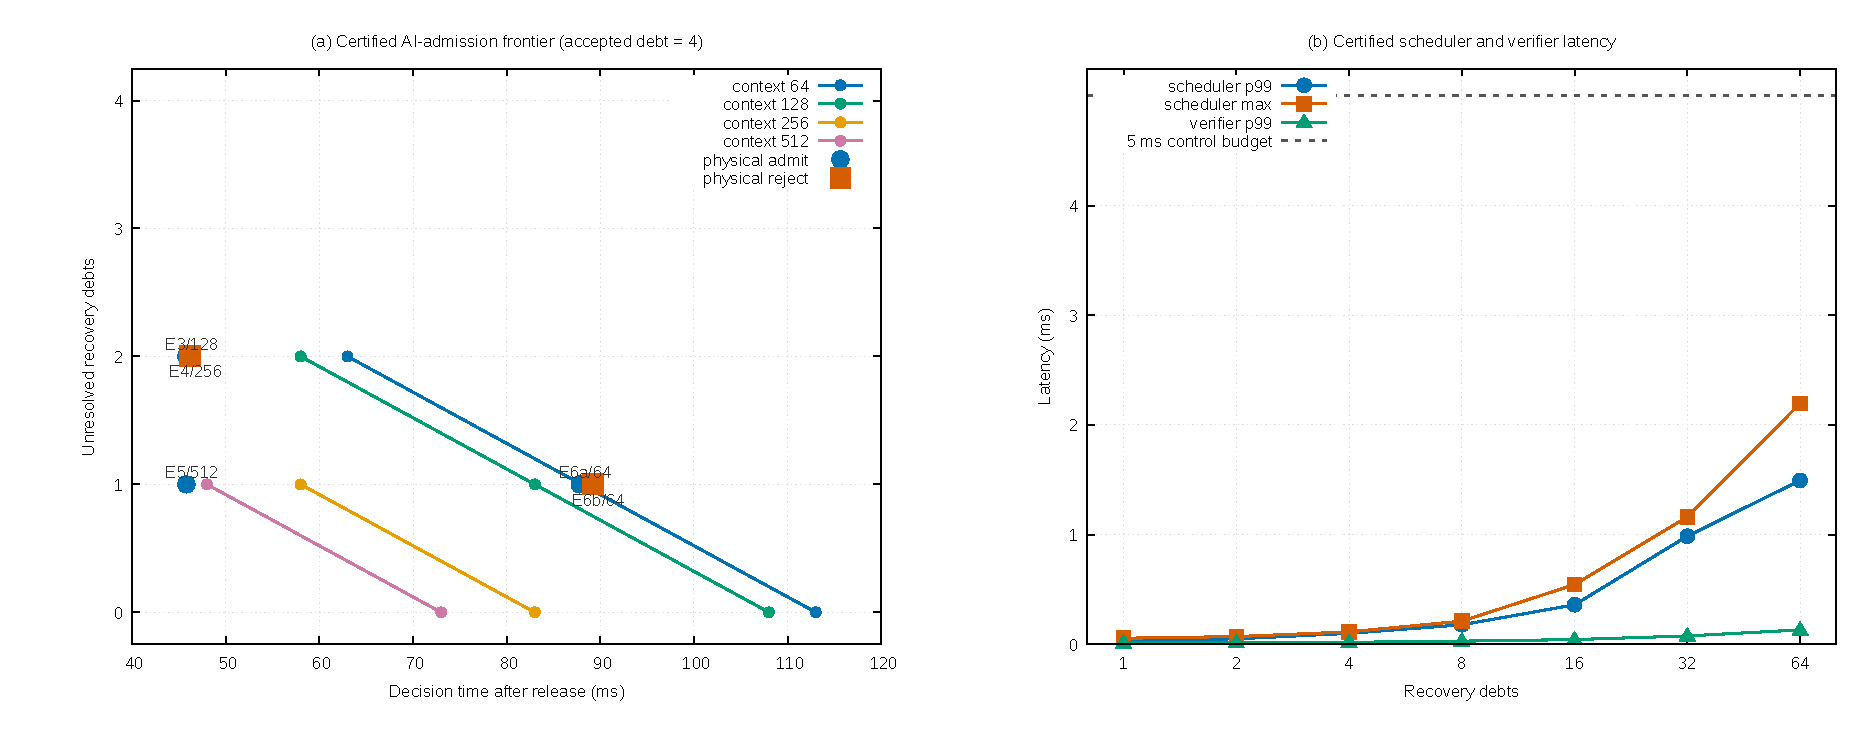
\includegraphics[width=\linewidth]{../../docs/current/figures/softwall_c162_envelope_scalability.pdf}
  \caption{Qualified AI-admission frontier versus debt, AI class, and decision time (a), and
  certified-scheduler latency through 64 debts (b). Prespecified physical cases lie on their predicted
  sides of the frontier. Latencies are finite-run measurements, not WCETs.}
  \Description{The first plot shows an AI-admission frontier moving with recovery debt and context
  size. The second shows scheduler and verifier latency through 64 debts with a five-millisecond
  control-budget reference.}
  \label{fig:envelope}
\end{figure}

\noindent\textbf{Answer to RQ4.}
Figure~\ref{fig:envelope} shows that the same AI class and debt can cross from \QSU to \QSN as the
decision time advances. The envelope predicts this transition without future CRC or realized service
time.

\subsection{Certified scheduler scalability}

RQ5 asks whether certificate construction remains useful beyond the state size handled by exact
search. Safety is delegated to the verifier; heuristic incompleteness may reject a feasible state but
cannot admit an invalid one.

% provenance: C162_SCHEDULER
\noindent\textbf{Exact Comparison.}
On 600 heterogeneous small states, exact search accepted 504 and the deterministic candidate accepted
494. False-safe was zero and false-conservative was ten. On the current qualified mode, candidate and
exact acceptance matched across all 16,023 states.

\noindent\textbf{Control-Path Cost.}
A 2,800-state grid spans 1-64 debts and capacities 1, 2, 4, and 8. Every returned certificate passed
the independent verifier. At 64 debts, candidate decision latency was 1.494~ms p99 and 2.197~ms
maximum; verifier p99 was 0.131~ms. These finite-run CPU measurements remain below the evaluated
control budget, but they are not WCETs.

\subsection{What the certificate prevents}

Proposition~2 concerns guarantee authority, not an instruction to manufacture deadline misses. RQ4's
prespecified boundary cases provide witnesses using declared service bounds.

% provenance: C162_NECESSITY
\noindent\textbf{False-Safe Witnesses.}
In E4, two debts remain at 45~ms and a context-256 request is visible. Mandatory-only recovery is
feasible, but debt-blind admission permits a bound-respecting completion at 165~ms, 12~ms beyond the
153~ms guard. In E6b, one debt remains and context-64 becomes unsafe at 89~ms; completion reaches
154~ms, one millisecond beyond the guard. \sys classified both states as \QSN and rejected all 30
requests per case across two nodes before launch.

\noindent\textbf{Interpretation.}
These are contract-level counterexamples. We do not label them observed debt-blind deadline misses
because the rejected kernels were not launched. The MPS-only results in Section~\ref{sec:eval-mps}
provide the separate evidence that physical cap-only tails can occur. Table~\ref{tab:necessity}
separates safety authority from AI-first utility.

\begin{table}[t]
\caption{Safety necessity and AI-first utility are different comparisons.}
\label{tab:necessity}
\begin{tabularx}{\linewidth}{@{}p{0.26\linewidth}p{0.16\linewidth}p{0.18\linewidth}X@{}}
\toprule
Policy & All-fail check & AI before debt clears & Finding \\
\midrule
Debt-blind current-idle & No & Yes & Cannot guarantee E4/E6b; unsafe diagnostic \\
Certificate-preserving recovery-first & Yes & No & Safe comparator; 385,262 timely tokens \\
\sys & Yes & Only with witness & Same 385,262 tokens; predicts the boundary \\
\bottomrule
\end{tabularx}
\end{table}

\noindent\textbf{Bound Sensitivity.}
The witnesses use the qualified $B_{\mathrm{conv}}=25$~ms contract. E6b disappears at or below 24~ms;
E4 remains until 19~ms, and only E4 remains false-safe for $19 < B_{\mathrm{conv}} \leq 24$~ms. The
observed recovery-path maximum was 13.465~ms, or 1.86$\times$ below the declared bound, but a sample
maximum cannot replace a service contract. A lower bound defines another mode and moves the false-safe
interval rather than making unresolved debt irrelevant. That new boundary requires requalification.

A failure-correlation sweep is unnecessary for the safety conclusion because the contract already
admits correlated all-fail behavior. Correlation affects expected utility, which RQ6 measures
separately.

\subsection{Strong baseline and no material headroom}

RQ6 tests whether AI-first retiming increases timely external-AI value over a safe policy that already
models recovery debt. It does not test whether certificates are necessary.

% provenance: C159_BASELINE
\noindent\textbf{Matched Comparison.}
The certificate-preserving recovery-first baseline and \sys share max-radio decisions, all-fail
admission, observable state, arrivals, service bounds, qualified workers, and single-commit behavior.
Their sole semantic difference is whether AI may execute before unresolved recovery physically
completes.

\noindent\textbf{Result.}
Four non-overlapping BurstGPT calibration windows contain 4,290 requests and 1,129,504 offered tokens.
Both systems complete 931 timely requests and 385,262 timely tokens. A sensitivity charging every
recovery its full 25~ms bound improves \sys's timely token value by 0.066\%, below the prespecified
5\% minimum effect. We did not open the confirmatory throughput holdout.

\noindent\textbf{Answer to RQ6.}
AI-first retiming does not increase timely tokens on this trace. The evaluated one-second AI SLO allows
recovery-first catch up. Conditional capacity and its safety boundary remain observable, but we make
no optimizer claim.

\subsection{Lifecycle qualification}

RQ7 begins by asking which process and worker lifecycles can use the qualified bounds. The matrix is
claim-scoped rather than a checklist to fill after observing results.

% provenance: C164_LIFECYCLE
\begin{table}[t]
\caption{Lifecycle envelope. ``Partial'' qualifies only the stated safe subset.}
\label{tab:lifecycle}
\begin{tabularx}{\linewidth}{@{}Xll@{}}
\toprule
Mode & Status & Claimed property \\
\midrule
Warm persistent & Qualified & Full evaluated contract \\
First request after 30~s idle & Qualified & Bounded first transaction \\
MPS restart + requalification & Partial & No reuse before requalification \\
Qwen reload & Partial & Mandatory radio continuity \\
Same-worker reconnect & Partial & Generation reconciliation \\
Process/model cold & \UQ & None \\
5~min idle & \UQ & None \\
30~min idle & \UQ & None \\
GC-on & \UQ & None \\
Worker process replacement & \UQ & Development canary only \\
\bottomrule
\end{tabularx}
\end{table}

\noindent\textbf{Qualified Subsets.}
The paper has five qualified or partial subsets and five \UQ modes. Qualified evidence covers warm
persistent execution, the first request after 30~s idle, MPS restart followed by requalification,
mandatory radio continuity during Qwen reload, and same-worker reconnect reconciliation. It does not
claim optional-service availability during restart or reload.

\noindent\textbf{Unqualified Lifecycles.}
Process/model cold, 5~min and 30~min idle, GC-on, and worker process replacement remain \UQ. A
single-node replacement development canary passed its internal gate but lacks an independent holdout.
Durable journal recovery would be a new mechanism and remains outside this paper.

\subsection{Production exit gates}

The synthetic contract does not establish production timing. We use a vendor integration threshold to
falsify candidate implementations while keeping target-DU timing as the first unresolved gate.

\noindent\textbf{Timing Contract.}
Aerial testMAC expects CRC-bearing UL indication by $T0+4.5$~ms. Its validator reconstructs slot $T0$
and marks later handler arrival as late. TestMAC is a controlled developer L2 rather than a field-DU
$d_{\mathrm{MAC}}$ source. The target-DU trace is absent, and we make no production HARQ guarantee.

% provenance: P2_FAST_PATH_AND_STAGE
\noindent\textbf{Path Elimination and Attribution.}
Under clean, warm, no-AI conditions, local wait-then-recover, same-GPU speculative, and precomputed
cross-GPU paths each complete 0/1,000 requests within 4.5~ms. Raw-IQ P2P moves channel estimation
through CRC to GPU1 and improves completion to 852/1,000 with 3.831~ms median. Binding cuPHY and
caller-owned TensorRT to one stream reaches 885/1,000 but retains 115 late samples. A 300-request
profile attributes that path's tail to remote channel estimation: GPU p50/p99/max are
0.866/4.873/9.592~ms and correlation with pair wall time is 0.9603. TensorRT host enqueue averages
7.443~$\mu$s, while its graph has 0.886~ms GPU p99. Forward/backward P2P copies average
36.261/17.150~$\mu$s. Derate-match host call averages 1,060.105~$\mu$s with 1,105.380~$\mu$s p99,
while its GPU p99 is 0.168~ms.

\noindent\textbf{Frozen Fast-Path Gate.}
We froze persistent Fortran-layout input and stream-ordered assembly as one bounded implementation
change. The development gate reaches 995/1,000 timely requests, with 3.813~ms median and 3.995~ms p99;
both decoders are correct for all requests. Five late completions reject the candidate and leave the
holdout closed. Four are limited by conventional completion and one by remote \NRx. Pair latency
correlates 0.918 with conventional GPU service and 0.3307 with remote \NRx. A conventional profile
identifies equalization as its strongest stage correlate ($r=0.761$; 1.904~ms maximum), while
conventional channel estimation reaches 1.295~ms. The remaining tail spans both cuPHY paths. These
profiles are mechanism evidence rather than qualification or WCET. The bounded P2 campaign stops at
this failed gate. The native C++ path establishes fixture and layout parity only and is not a timing
qualification.

\subsection{Supported-channel \NRx result}

The final part of RQ7 asks whether optional \NRx provides conditional radio value under a declared
external channel contract. Unsupported and supported domains are both reported.

\noindent\textbf{External Aerial TDL-A.}
Across raw and normalized inputs, public-reference radio settings, one-antenna frequency/time channel
execution, and a public-notebook-style FP32 engine, conventional decoding succeeds in every ten-TB
arm and \NRx succeeds in none. TDL-A remains \UQ.

% provenance: P3_CHANNEL_HOLDOUT
\noindent\textbf{Frozen Sionna Holdout.}
We reconstruct the Sionna 1.0.2/TensorFlow 2.19 contract. Clean MCS7 and Rayleigh controls pass, and a
fixed development matrix selects CDL-D/E at 100~ns while retaining A/B/C failures. A disjoint-seed
holdout uses new payload, slot, and channel seeds across five Es/No strata and 50 blocks per stratum
per model. Both pipelines pass 50/50 at 10~dB. Table~\ref{tab:channel-holdout} reports all paired
outcomes.

\begin{table}[t]
\caption{Frozen disjoint-seed Sionna CDL-D/E holdout.}
\label{tab:channel-holdout}
\begin{tabularx}{\linewidth}{@{}Xrrrr@{}}
\toprule
Mode & Conv. & \NRx & \NRx-only & Conv.-only \\
\midrule
CDL-D, 100~ns & 153/250 & 164/250 & 16 & 5 \\
CDL-E, 100~ns & 155/250 & 163/250 & 15 & 7 \\
Paired aggregate & -- & -- & \textbf{31} & \textbf{12} \\
\bottomrule
\end{tabularx}
\end{table}

\noindent\textbf{Channel Claim.}
The aggregate discordant outcomes give a two-sided exact $p=0.00540$. The optional \NRx has conditional radio value
in this frozen Sionna CDL-D/E mode. The result qualifies neither Aerial TDL-A nor field IQ,
and the channel mode has not passed production timing or integrated service-vector qualification.

\section{Related Work}

Prior systems establish the mechanisms on which \sys builds: AI-and-RAN resource allocation,
deadline-aware accelerator selection, GPU slack reclamation, and AI/conventional PHY choice. Our
comparison asks a narrower question: whether the scheduler represents the unresolved conventional
obligation created by an optional receiver for the same TB. Table~\ref{tab:closest} summarizes this
distinction at the level of the protected object.

\begin{table}[t]
\caption{Closest-work distinction. ``Not exposed'' describes the public design and is not a claim that
the mechanism could never be extended.}
\label{tab:closest}
\begin{tabularx}{\linewidth}{@{}p{0.20\linewidth}p{0.29\linewidth}X@{}}
\toprule
System & Primary protected/allocated object & State not exposed to its scheduler \\
\midrule
YinYangRAN & MPS fraction and CPU fallback & Multi-cell unresolved same-TB recovery calendar \\
CloudRIC & Queued request and accelerator deadline & Recovery jobs that have not entered a queue \\
Concordia & Reserved/reclaimed vRAN CPU capacity & Optional-PHY outcome-conditioned debt \\
DARIS, REEF, XSched, nvtaskset & GPU stage, kernel, context, or partition & Radio recovery, transport ownership, and single commit as one certificate \\
ARCHES, OCUDU & AI/conventional PHY selection or timing class & Cross-home all-fail debt plus atomic external-AI lease \\
SMEC & RAN/edge SLO coordination & Same-PHY-GPU optional receiver recovery \\
\sys & Same-TB recovery obligation & Explicitly modeled, certified, and carried through physical completion \\
\bottomrule
\end{tabularx}
\end{table}

\subsection{AI-and-RAN resource allocation}

AI-and-RAN systems already allocate heterogeneous compute across radio and external-AI demand. They
establish that dynamic sharing and deadline-aware placement are useful; their public scheduling state
does not expose a future same-TB recovery job before that job enters an execution queue.

\noindent\textbf{Shared Acceleration.}
YinYangRAN adjusts MPS fractions between PHY and ML and can use CPU fallback~\cite{yinyangran}.
CloudRIC places RAN requests across heterogeneous accelerators from queue and deadline
estimates~\cite{cloudric}. These systems establish MPS-based sharing, fallback, and deadline-aware
accelerator selection as prior art. \sys does not claim any of those mechanisms.

\noindent\textbf{Placement and Orchestration.}
Interplay and CAORA use learning-based orchestration and MIG allocation~\cite{interplay,caora}; HAF
separates slow placement from fast deadline-aware CPU/GPU allocation~\cite{haf}. A distributed AI-RAN
platform addresses placement across RAN sites~\cite{distributedairan}. Their allocation units are
workers, resources, or queued jobs. \sys represents the conventional recovery of an unresolved
optional receiver as mandatory future work tied to one radio result.

\subsection{GPU slack and real-time execution}

Resource reclamation and GPU execution control explain how lower-priority work can coexist with a
latency-sensitive tenant. \sys uses these mechanisms, while its certificate protects a radio-specific
obligation that spans scheduler state, transport ownership, and physical completion.

\noindent\textbf{Slack Reclamation.}
Concordia reserves CPU capacity for vRAN and reclaims the remainder~\cite{concordia}. DARIS combines
MPS, streams, and stage boundaries to admit lower-priority DNN work~\cite{daris}. Their reclaimed
capacity is derived from a reservation or an execution-stage boundary. Recovery debt changes when an
optional outcome resolves and must remain feasible under a correlated all-fail branch.

\noindent\textbf{GPU Execution Control.}
REEF, XSched, and nvtaskset provide preemption, isolation, or context-scheduling
mechanisms~\cite{reef,xsched,nvtaskset}. These controls can reduce interference, but they do not by
themselves bind an admission decision to launch-time revalidation, endpoint ownership, CUDA
completion, and a single radio commit. The seven counterexamples in
Section~\ref{sec:requirements} motivate that refinement chain.

\subsection{AI/conventional PHY paths and MEC scheduling}

Neural/conventional PHY coexistence and 5G-aware application scheduling are also established ideas.
The relevant distinction is whether optional decoding creates a multi-cell recovery obligation on the
same GPU that also runs external AI.

\noindent\textbf{PHY Path Selection.}
ARCHES selects neural or conventional PHY experts according to channel conditions~\cite{arches}.
OCUDU exposes in-DU AI-RAN timing classes, retains a conventional path, and validates result and
lifecycle behavior~\cite{ocudu}. These works rule out novelty claims for neural/conventional
coexistence, fallback, or timing classes. Their public designs do not present the combination of a
multi-cell all-fail recovery calendar and an atomic external-AI lease carried to a physical fence.

\noindent\textbf{Edge SLO Coordination.}
SMEC coordinates application SLOs through decoupled RAN and edge schedulers and uses MPS priority at
the MEC GPU~\cite{smec}. Its AI work executes on a separate edge server rather than the PHY GPU that
holds optional same-TB recovery. \sys makes no novelty claim for 5G-aware deadline scheduling.

\noindent\textbf{Scoped Difference.}
Across the public designs reviewed through September 2026, we did not find a system that combines
three properties: an executable all-fail calendar for unresolved same-TB recovery, atomic leasing of
the remaining capacity to external AI through physical retirement, and a provenance-qualified
predictive feasibility envelope. This statement is a scoped literature finding, not proof about
unpublished work or work using different terminology.

\section{Limitations}

The evaluation deliberately separates a qualified synthetic contract from production timing, and a
supported simulated channel from unqualified radio domains. These boundaries determine where the
current evidence can be used.

\subsection{Timing contract and statistical bounds}

The measured modes establish finite-sample qualification on one hardware family. They do not convert
the synthetic harness into a production radio deadline or a probabilistic sample maximum into a
worst-case execution-time bound.

\noindent\textbf{Production Timing.}
\texttt{P180/D155} is a synthetic harness contract: $P$ is the inter-release period, not an NR slot
duration, and \texttt{D155} is not a production HARQ deadline. The production \texttt{d\_MAC} trace
builder, clock and provenance checks, request-specific exact/certified bridge, and expiry validator
are implemented and pass 24 unit tests, but a target DU/FAPI trace is unavailable. A new timing vector
would require physical requalification. Aerial testMAC supplies a $T0+4.5$\,ms developer-L2
threshold; the best raw-IQ two-GPU candidate reaches only 995/1,000 clean requests and fails its frozen
gate. We make no production HARQ guarantee.

\noindent\textbf{Finite-Sample Qualification.}
Zero observed violations under a qualified mode do not establish WCET or zero failure probability.
Each bound belongs to its hardware, software, placement, workload, and lifecycle fingerprint. A
changed fingerprint defines another mode and must pass the same prediction and physical gates.

\noindent\textbf{Hardware Scope.}
All authoritative hardware results use the NVIDIA A100 family. The four-GPU and multi-home paths
exercise NVLink P2P, but the evidence does not establish cross-family or inter-node data-plane
validity.

\subsection{Fault and lifecycle coverage}

The fault model closes bounded response, ownership, and worker-transition cases. Arbitrary GPU or
driver hangs and durable recovery after full worker replacement remain outside the qualified set.

% provenance: C158_LONG_TAIL
\noindent\textbf{Unresolved Long Tail.}
In C158 attempt 4, one \NRx completion reached 350.948\,ms in a 400-request run whose \NRx p99 was
8.111\,ms, a 43.3$\times$ excursion; the run consequently had 4/400 deadline misses. Targeted
30\,s-idle, quiescent MPS-restart/requalification, Qwen-reload, and same-worker reconnect campaigns
did not reproduce the event. Its root cause remains unresolved, and those lifecycle results do not
qualify the tail away.

\noindent\textbf{Unqualified Lifecycles.}
Five lifecycle modes remain \UQ, including full worker replacement. The runtime fails closed when a
fence or ownership transition is unresolved. Durable journal recovery would introduce a new mechanism
rather than complete evidence for the current one.

\subsection{PHY and workload generality}

The qualified result covers one standardized simulated-channel mode and one representative external-AI
trace mapping. It does not establish field-channel generalization or a universal throughput benefit.

\noindent\textbf{Channel Domain.}
External Aerial TDL-A development screens retain conventional success on every ten-TB arm and \NRx
success on none across normalization, public-reference radio parameters, exact one-antenna
transmission, frequency/time channel execution, and FP32 engine precision. A frozen Sionna CDL-D/E
holdout passes its high-SNR pipeline and conditional-value gates over 500 paired blocks, with 31
\NRx-only and 12 conventional-only low-SNR outcomes. This qualifies only that simulated CDL-D/E mode;
it does not establish Aerial TDL-A, recorded field IQ, or over-the-air behavior. The supported channel
has not traversed production timing and integrated service-vector qualification.

\noindent\textbf{External-AI Mapping.}
BurstGPT supplies real request arrivals and token lengths, while Qwen2.5-1.5B prefill is a
representative external workload rather than an AI-RAN domain application. Token bucketing and the
one-second deadline are experimental mappings. Different model architectures, generation phases, or
independently justified SLOs require new service bounds and replay qualification.

\noindent\textbf{Utility Scope.}
The strongest safe comparison finds no material throughput advantage. Selecting a tighter AI
deadline after observing that result would be post hoc. The demonstrated operational value is advance
classification of safe, no-slack, infeasible, and unqualified modes, together with rejection of work
that would break a certificate. The paper therefore makes a substrate and envelope claim.

\section{Conclusion}

Optional \NRx creates mandatory future work that current GPU idleness does not expose. \sys represents
that work as recovery debt, maintains an executable multi-cell all-fail certificate, and admits
external AI through a transaction that remains valid across control, transport, launch, and physical
completion. Seven measured counterexamples derive the refinement chain, and the predictive envelope
classifies a qualified mode before the corresponding physical outcome is opened.

Across two independent A100 nodes, the evaluated modes exercise actual \NRx, shared cuPHY recovery,
Qwen execution, multi-GPU transfers, and bounded fault transitions. The same evaluation finds no
material AI-first throughput gain over a certificate-preserving recovery-first baseline and rejects
the production fast-path candidate at 995/1,000. The supported claim is therefore precise: SoftWall
provides a conditional-recovery substrate and feasibility envelope for qualified modes; finite
samples, unsupported channels, and the absent target-DU timing contract do not establish WCET or a
production HARQ guarantee.

\bibliographystyle{ACM-Reference-Format}
\bibliography{references}

\end{document}
